\documentclass{beamer}

\usepackage{graphicx, amssymb, listings}
%\usepackage[active]{srcltx}
%\usepackage[all,xdvi]{xy}
%\usepackage{showlabels}
\usepackage[alphabetic,y2k,lite]{amsrefs}

%%%%%%%%%%%%%%%%%% Tikz %%%%%%%%%
\usepackage{tikz}
\usetikzlibrary{shapes.geometric}
\usetikzlibrary{calc}
\usetikzlibrary{scopes}
\usetikzlibrary{decorations.markings}
%\usepackage[labelformat=empty]{caption}

\tikzset{
every picture/.style={line width=0.8pt, >=stealth,
                       baseline=-3pt,label distance=-3pt},
%%%%%%%%%%  Node styles
dotnode/.style={fill=black,circle,minimum size=2.5pt, inner sep=1pt, outer
sep=0},
morphism/.style={circle,draw,thin, inner sep=1pt, minimum size=15pt,
                 scale=0.8},
small_morphism/.style={circle,draw,thin,inner sep=1pt,
                       minimum size=10pt, scale=0.8},
coupon/.style={draw,thin, inner sep=1pt, minimum size=18pt,scale=0.8},
%%%% different line styles:
regular/.style={densely dashed},
edge/.style={thick, dashed, draw=blue, text=black},
boundary/.style={thick,  draw=blue, text=black},
overline/.style={preaction={draw,line width=2mm,white,-}},
drinfeld center/.style={>=stealth,green!60!black, double
distance=1pt,text=black},
%%%%%%% Fill styles %%%%%%%%%%%%%%%
cell/.style={fill=black!10},
subgraph/.style={fill=black!30},
%%%%%%% Mid-path arrows
midarrow/.style={postaction={decorate},
                 decoration={
                    markings,% switch on markings
                    mark=at position #1 with {\arrow{>}},
                 }},
midarrow/.default=0.5
}
%%%%%%%%%%%%%%%%%%%%%%%%%%%%%%%%%%%%%%%%

\newcommand{\ph}{\varphi}
\renewcommand{\Im}{\mathrm{Im}}

\newcommand{\ee}{\mathbf{e}}
\DeclareMathOperator{\Obj}{Obj}
\DeclareMathOperator{\FPdim}{FPdim}
\DeclareMathOperator{\Hom}{Hom}
\DeclareMathOperator{\ev}{ev}
\DeclareMathOperator{\coev}{coev}
\DeclareMathOperator{\id}{id}
\DeclareMathOperator{\End}{End}
\DeclareMathOperator{\MCG}{MCG}
\DeclareMathOperator{\Homeo}{Homeo}
\DeclareMathOperator{\Vect}{Vect}
\DeclareMathOperator{\Mod}{Mod}
\DeclareMathOperator{\PGL}{PGL}

\newtheorem{prop}[theorem]{Proposition}
\newtheorem{conj}[theorem]{Conjecture}


\newcommand{\img}[1]{
\vfill
\centering
\includegraphics[width=\textwidth,height=0.8\textheight,keepaspectratio]{#1}
\vfill
} 

% There are many different themes available for Beamer. A comprehensive
% list with examples is given here:
% http://deic.uab.es/~iblanes/beamer_gallery/index_by_theme.html
% You can uncomment the themes below if you would like to use a different
% one:
%\usetheme{AnnArbor}
%\usetheme{Antibes}
%\usetheme{Bergen}
%\usetheme{Berkeley}
%\usetheme{Berlin}
%\usetheme{Boadilla}
%\usetheme{boxes}
%\usetheme{CambridgeUS}
%\usetheme{Copenhagen}
%\usetheme{Darmstadt}
%\usetheme{default}
%\usetheme{Frankfurt}
%\usetheme{Goettingen}
%\usetheme{Hannover}
%\usetheme{Ilmenau}
%\usetheme{JuanLesPins}
%\usetheme{Luebeck}
%\usetheme{Madrid}
%\usetheme{Malmoe}
%\usetheme{Marburg}
%\usetheme{Montpellier}
%\usetheme{PaloAlto}
%\usetheme{Pittsburgh}
%\usetheme{Rochester}
\usecolortheme{seahorse}
%\usetheme{Singapore}
%\usetheme{Szeged}
%\usetheme{Warsaw}

\title{On the Property F Conjecture}
\date{Paul Gustafson \\ Texas A\&M University}

\begin{document}
\frame{\titlepage}

\begin{frame}{Outline}
  \begin{itemize}
  \item The Property F conjecture for mapping class groups
  \item Proof in $\Vect_G^\omega$ case
  \item Progress in the metaplectic case
  \end{itemize}
\end{frame}


\begin{frame}{Definition of the mapping class group}
\begin{itemize}
\item
    Let $\Sigma = \Sigma_{g,b}^m$ be the oriented compact surface of genus $g$ with $b$ boundary components and $m$ marked points in its interior.

    \pause
\item
   The mapping class group of $\Sigma$, 
   $MCG(\Sigma),$
   is the group of isotopy classes of orientation-preserving homeomorphisms of $\Sigma$ that preserve the boundary \emph{pointwise} and preserve the marked points \emph{setwise}.

  \item Examples
  \begin{itemize}
    \item $\MCG(\Sigma_{0,1}^m) = B_m$
    \item $\MCG(\Sigma_{1,0}^0) = SL(2,\mathbb Z)$
  \end{itemize}
\end{itemize}
\end{frame}


\begin{frame}{The Property F conjecture}
\begin{conj}[Rowell]
Braiding an anyon $X$ is universal iff $\dim(X)^2 \not\in \mathbb{Z}$.
\end{conj}

\begin{itemize}
\item Verified for modular categories from quantum groups (Rowell, Naidu, Freedman, Larsen, Wang, Wenzl, Jones, Goldschmidt)
\end{itemize}
\end{frame}



\begin{frame}{A conjecture for mapping class groups}
\begin{conj}
The Turaev-Viro-Barrett-Westbury (TVBW) mapping class group representation associated to a compact surface $\Sigma$ and spherical fusion category $\mathcal A$ has finite image iff $\mathcal A$ is weakly integral.
\end{conj}

\vspace{0.2in}

\begin{itemize}
\pause
\item In this talk: $\mathcal A = \Vect_G^\omega$ -- the category of $G$-graded vector spaces with associativity twisted by a 3-cocycle $\omega$ 
\item This is the same as the twisted Dijkgraaf-Witten TQFT
\end{itemize}

\end{frame}


\begin{frame}{Related Work}
\begin{theorem}[Etingof--Rowell--Witherspoon]
The braid group representation associated to 
the modular category $\Mod(D^\omega(G))$ has finite image.
\end{theorem}

\begin{theorem}[Fjelstad--Fuchs]
Every mapping class group representation of a closed surface with at most one marked point associated to $\Mod(D(G))$ has finite image.
\end{theorem}

% ng schaumburg - genus 1, any modular category
\begin{theorem}[Ng--Schauenberg]
Every representation of $SL(2,\mathbb{Z})$ associated to a modular category has finite image.
\end{theorem}
\end{frame}


\begin{frame}{The spherical fusion category $\Vect^\omega_G$}
  The spherical fusion category $\Vect^\omega_G$ is the category of $G$-graded finite-dimensional vector spaces with the following structural morphisms, where $V_g$ is the simple object:   
\begin{itemize} 
\item The associator $\alpha_{g,h,k}:(V_g \otimes V_h) \otimes V_k \to V_g \otimes (V_h \otimes V_k)$
            $$ \alpha_{g,h,k} = \omega(g,h,k)$$
\item The evaluator $\ev_g:V_g^* \otimes V_g \to 1$
  $$ ev_g = \omega(g^{-1},g,g^{-1})$$
\item The coevaluator $\coev_g:V_g \otimes V_g^* \to 1$
    $$\coev_g = 1$$
\item The pivotal structure $j_g:V_g^{**} \to V_g$
            $$ j_g = \omega(g^{-1},g,g^{-1})$$
\end{itemize}

\end{frame}


\begin{frame}{Main result}
\begin{theorem}[G]
The image of any $\Vect^\omega_G$ TVBW representation $\rho$ of a mapping class group of an orientable, compact surface $\Sigma$ with boundary is finite.
\end{theorem}
Proof outline:
\begin{itemize}
  \item Describe a tractable presentation of  the representation space
  \item Find a good finite spanning set $S$ for the representation space
  \item Calculate the action of each Birman generator on $S$
  \item Show that the representation of each Birman generator lies in a quotient of a finite group of monomial matrices.  
\end{itemize}
\end{frame}

\begin{frame}{Proof outline}
\begin{itemize}
  \item Describe a tractable presentation of  the representation space
\end{itemize}
\end{frame}

\begin{frame}{The TVBW space associated to a 2-manifold}
  \begin{itemize}
    \item 
        Kirillov: The TVBW representation space is canonically isomorphic to
        \[
        H := \frac{\text{formal linear combinations of $\mathcal A$-colored graphs in $\Sigma$}  }
        {\text{local relations}}
       \]
  \end{itemize}

\end{frame}

\begin{frame}{Colored graphs in $\Sigma$}
\begin{itemize}
\item Let $\Gamma \subset \Sigma$ be an undirected finite graph embedded in $\Sigma$.

\pause \item Define $E^{or}$ to be the set of orientation edges of $\Gamma$, i.e. pairs $\ee=(e,\text{orientation of } e)$; for such an oriented edge $\ee$, we denote by $\bar{\ee}$ the edge with opposite orientation. 

\pause \item A {\em coloring} of $\Gamma$ is the
following data: 
\begin{itemize}
    \item Choice of an object $V(\ee)\in \Obj \mathcal A$ for every oriented edge  $\ee \in E^{or}$ so that $V(\bar{\ee})=V(\ee)^*$.
    \pause \item Choice of a vector $\ph(v)\in \Hom_{\mathcal A}(1, V_1 \otimes \cdots \otimes V_n)$  for  every interior vertex $v$, where 
      $\ee_1, \dots, \ee_n$ are edges incident to $v$, taken in counterclockwise
      order and with outward orientation.
\end{itemize}
\end{itemize}
\end{frame}


\begin{frame}{Local relations}
\begin{itemize}
\item Isotopy of the graph embedding
\item Linearity in the vertex colorings
\item The following three relations:
\end{itemize}

\begin{figure}[ht]
%%%%%%%%%%%%%%%%%%%%%%%%%%%%%%%%%%%%%%%%%%%%%%%%%%%%%%%
%%%%%%%%%%

\begin{tikzpicture}
\node[morphism] (ph) at (0,0) {$\ph$};
\node[morphism] (psi) at (1,0) {$\psi$};
\node at (-0.7,0.1) {$\vdots$};
\node at (1.7,0.1) {$\vdots$};
\draw[->] (ph)-- +(220:1cm) node[pos=1.0,below,scale=0.8]
{$V_n$};
\draw[->] (ph)-- +(140:1cm) node[pos=1.0,above,scale=0.8]
{$V_1$};
\draw[->] (psi)-- +(40:1cm) node[pos=1.0,above,scale=0.8]
{$W_m$};
\draw[->] (psi)-- +(-40:1cm) node[pos=1.0,below,scale=0.8]
{$W_1$};
\draw[->] (ph) -- (psi) node[pos=0.5,above,scale=0.8] {$X$};
\end{tikzpicture}
%%%%%%%%
=
%%%%%%%%
\begin{tikzpicture}
\node[ellipse, thin, scale=0.8, inner sep=1pt, draw] (ph) at (0,0)
             {$\ph\circ_{X}\psi$};
\node at (-0.8,0.1) {$\vdots$};
\node at (0.8,0.1) {$\vdots$};
\draw[->] (ph)-- +(220:1cm) node[pos=1.0,below,scale=0.8] {$V_n$};
\draw[->] (ph)-- +(140:1cm) node[pos=1.0,above,scale=0.8] {$V_1$};
\draw[->] (ph)-- +(40:1cm) node[pos=1.0,above,scale=0.8]  {$W_m$};
\draw[->] (ph)-- +(-40:1cm) node[pos=1.0,below,scale=0.8] {$W_1$};
\end{tikzpicture}
%%%%%%%%%
\\
%%%%%%%%%
\begin{tikzpicture}
\node[dotnode] (ph) at (0,0) {};
\node[dotnode] (psi) at (1.5,0) {};
\node at (-0.7,0.1) {$\vdots$};
\node at (2.2,0.1) {$\vdots$};
\draw[->] (ph)-- +(220:1cm) node[pos=1.0,below,scale=0.8] {$A_n$};
\draw[->] (ph)-- +(140:1cm) node[pos=1.0,above,scale=0.8] {$A_1$};
\draw[->] (psi)-- +(40:1cm) node[pos=1.0,above,scale=0.8] {$B_m$};
\draw[->] (psi)-- +(-40:1cm) node[pos=1.0,below,scale=0.8] {$B_1$};
\draw[out=45,in=135, midarrow] (ph) to (psi)
                node[above,xshift=-0.6cm, yshift=0.25cm, scale=0.8] {$V_k$};
\draw[ out=15,in=165, midarrow] (ph) to (psi);
\draw[ out=-15,in=195, midarrow] (ph) to (psi);
\draw[ out=-45,in=225, midarrow] (ph) to (psi) node[below, xshift=-0.6cm, yshift=-0.3cm, scale=0.8] {$V_1$};
\end{tikzpicture}
%%%%%%%%%%%
=
%%%%%%%%%%%
\begin{tikzpicture}
\node[dotnode] (ph) at (0,0) {};
\node[dotnode] (psi) at (1.5,0) {};
\node at (-0.7,0.1) {$\vdots$};
\node at (2.2,0.1) {$\vdots$};
\draw[->] (ph)-- +(220:1cm) node[pos=1.0,below,scale=0.8] {$A_n$};
\draw[->] (ph)-- +(140:1cm) node[pos=1.0,above,scale=0.8] {$A_1$};
\draw[->] (psi)-- +(40:1cm) node[pos=1.0,above,scale=0.8] {$B_m$};
\draw[->] (psi)-- +(-40:1cm) node[pos=1.0,below,scale=0.8] {$B_1$};
\draw[ ->] (ph) to (psi)
            node[above,xshift=-0.8cm,scale=0.8] {$V_1\otimes \dots\otimes V_k$};
\end{tikzpicture}
%%%%%%%
\qquad $k\ge 0$
\\
%%%%%%%
\begin{tikzpicture}
\node[ellipse, scale=0.8, inner sep=1pt, draw,thin] (ph) at (0,0)
{$\mathrm{coev}$};
\draw[->] (ph)-- +(180:1cm) node[pos=1.0,above,scale=0.8] {$V$};
\draw[->] (ph)-- +(0:1cm) node[pos=1.0,above,scale=0.8] {$V^*$};
\end{tikzpicture}
%%%%%%%%
=
%%%%%%%%
\begin{tikzpicture}
\draw[->] (2,0)-- (0,0) node[pos=0.5,above,scale=0.8] {$V$};
\end{tikzpicture}
%%%%%%%%%%%%%%%%%%%%%%%%%%

\end{figure}

\end{frame}

\begin{frame}{Consequences of the local relations}

\begin{figure}[ht]
%%%%%%%%%%%%
\begin{tikzpicture}
\node[morphism] (ph) at (0,0) {$\ph$};
\node[morphism] (psi) at (1.5,0) {$\psi$};
\node at (-0.7,0.1) {$\vdots$};
\node at (2.2,0.1) {$\vdots$};
\draw[->] (ph)-- +(220:1cm) node[pos=1.0,below,scale=0.8] {$V_n$};
\draw[->] (ph)-- +(140:1cm) node[pos=1.0,above,scale=0.8] {$V_1$};
\draw[->] (psi)-- +(40:1cm) node[pos=1.0,above,scale=0.8] {$W_m$};
\draw[->] (psi)-- +(-40:1cm) node[pos=1.0,below,scale=0.8] {$W_1$};
\draw[->] (ph) -- (psi) node[pos=0.5,above,scale=0.8] {$X_1\oplus X_2$};
\end{tikzpicture}
%%%%%%%%%%%%
=
%%%%%%%%%%%%
\begin{tikzpicture}
\node[morphism] (ph) at (0,0) {$\ph_1$};
\node[morphism] (psi) at (1.5,0) {$\psi_1$};
\node at (-0.7,0.1) {$\vdots$};
\node at (2.2,0.1) {$\vdots$};
\draw[->] (ph)-- +(220:1cm) node[pos=1.0,below,scale=0.8]{$V_n$};
\draw[->] (ph)-- +(140:1cm) node[pos=1.0,above,scale=0.8]{$V_1$};
\draw[->] (psi)-- +(40:1cm) node[pos=1.0,above,scale=0.8]{$W_m$};
\draw[->] (psi)-- +(-40:1cm) node[pos=1.0,below,scale=0.8]{$W_1$};
\draw[->] (ph) -- (psi) node[pos=0.5,above,scale=0.8] {$X_1$};
\end{tikzpicture}
%%%%%%%%%%%%
+
%%%%%%%%%%%%
\begin{tikzpicture}
\node[morphism] (ph) at (0,0) {$\ph_2$};
\node[morphism] (psi) at (1.5,0) {$\psi_2$};
\node at (-0.7,0.1) {$\vdots$};
\node at (2.2,0.1) {$\vdots$};
\draw[->] (ph)-- +(220:1cm) node[pos=1.0,below,scale=0.8]{$V_n$};
\draw[->] (ph)-- +(140:1cm) node[pos=1.0,above,scale=0.8]{$V_1$};
\draw[->] (psi)-- +(40:1cm) node[pos=1.0,above,scale=0.8]{$W_m$};
\draw[->] (psi)-- +(-40:1cm) node[pos=1.0,below,scale=0.8]{$W_1$};
\draw[->] (ph) -- (psi) node[pos=0.5,above,scale=0.8] {$X_2$};
\end{tikzpicture}
%%%%%%%%%%%%


\caption{Additivity in edge colorings. Here $\ph_1,\ph_2$ are compositions
of $\ph$ with projector $X_1\oplus X_2\to X_1$ (respectively, 
$X_1\oplus X_2\to X_2$), and similarly for $\psi_1,\psi_2$.
}
\end{figure}

\begin{itemize}
\item Additivity in edge colorings
\end{itemize}

  \begin{theorem}[Kirillov, Reshitikhin--Turaev]
  A colored graph $\Gamma$ may be evaluated on any disk $D\subset \Sigma$, giving
  an equivalent colored graph $\Gamma'$ such that $\Gamma'$ is identical
  to $\Gamma$ outside of $D$, has the same colored edges crossing $\partial D$,
  and contains at most one colored vertex within $D$.
  \end{theorem}

\end{frame}


\begin{frame}{Proof outline}
\begin{itemize}
  \item Describe a tractable presentation of  the representation space
  \item Find a good finite spanning set $S$ for the representation space
\end{itemize}
\end{frame}

\begin{frame}{Spanning set for the representation space}
  By applying the local moves and the preceding theorem, any such representation space has a finite spanning set of ``simple'' colored graphs with a single vertex, loops for each of the standard generators of $\pi_1(\Sigma)$, and a leg from the vertex to each of the boundary components.  

\newdimen\R
\R=0.7cm
  
\begin{figure}
   \centering
    \begin{tikzpicture}[scale=3]    

      \draw (0:\R) \foreach \x in {45,90,...,359} {
                -- (\x:\R)
            } -- cycle;
      
                 
    \begin{scope}[very thick,decoration={
    markings,
    mark=at position 0.5 with {\arrow{>}}}
    ]  
      \draw[postaction={decorate}]  (0, 0) --  (22: {0.923879*\R}) node[pos=.5,sloped,above]{$g$};
      \draw[postaction={decorate}]  (0, 0) --  (67: {0.923879*\R}) node[pos=.5,above]{$h$};
      \draw[postaction={decorate}]  (112: {0.923879*\R}) -- (0, 0) node[pos=.5,above]{$g$};
      \draw[postaction={decorate}]  (157: {0.923879*\R}) -- (0, 0) node[pos=.5,sloped,above]{$h$};
      \draw[postaction={decorate}]  (0, 0) --  (202: {0.923879*\R}) node[pos=.5,sloped,above]{$k$};
      \draw[postaction={decorate}]  (0, 0) --  (247: {0.923879*\R}) node[pos=.5,sloped,above]{$l$};
      \draw[postaction={decorate}]  (292: {0.923879*\R}) -- (0, 0) node[pos=.5,sloped,above]{$k$};
      \draw[postaction={decorate}]  (337: {0.923879*\R}) -- (0, 0) node[pos=.5,sloped,above]{$l$};
    \end{scope}
    \end{tikzpicture}
%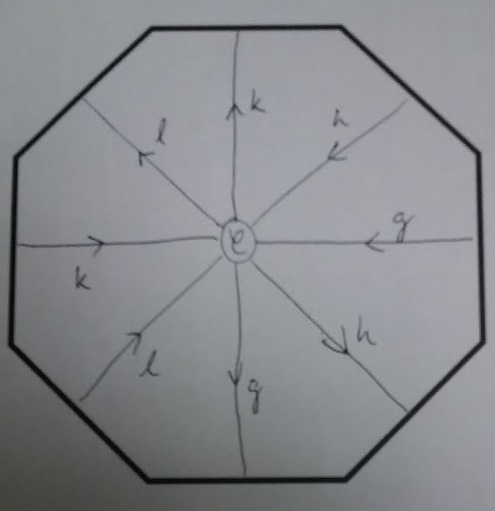
\includegraphics[width=0.5\textwidth]{basis.jpg}
\caption{Element of the spanning set for a genus 2 surface.  Here $[g,h][k,l] = 1$, and the vertex is labeled by a ``simple'' morphism (a $|G|$-th root of unity times a canonical morphism)}
\label{fig:span}
\end{figure}
\end{frame}


\begin{frame}{Proof outline}
\begin{itemize}
  \item Describe a tractable presentation of  the representation space
  \item Find a good finite spanning set $S$ for the representation space
  \item Calculate the action of each Birman generator on $S$
\end{itemize}
\end{frame}


\begin{frame}{Applying the Birman generators to the spanning set}
\begin{itemize}
\item  The next step of the proof is to apply each Birman generator to each element of the spanning set.
\item  In each case, we relate the resulting colored graph to another element of the spanning set by means of local moves
\item  The local moves map simple colored graphs to simple colored graphs
\item Hence, the Birman generators preserve the finite spanning set.
\end{itemize}
\end{frame}

%% \begin{frame}{Applying the Birman generators to the spanning set}
%% \begin{prop}[G.]
%% Let $\Gamma$ be a simple colored graph embedded in a surface $\Sigma$.  Let $\Delta$ be the colored graph given by applying one of the three local moves in Figure \ref{f:local_rels1} to $\Gamma$.  Then
%% \begin{enumerate}
%% \item  each edge of $\Delta$ is labeled by $\delta_g$ for some $g \in G$, and
%% \item  there exists $\alpha \in \mu_{|G|}$ such that 
%% $$\Delta = \alpha \Delta' $$
%% in $H$, where $\Delta'$ is a simple colored graph given by replacing each vertex label in $\Delta$ with a simple morphism.
%% \end{enumerate}
%% \end{prop}
%% \end{frame}
  
\begin{frame}{First Dehn twist}
\img{t1}
\end{frame}

\begin{frame}{Second Dehn twist}
\img{t2}
\end{frame}

\begin{frame}{Braid generator}
\img{t3}
\end{frame}

\begin{frame}{Dragging a point}
\img{t4}
\end{frame}

\newcommand{\one}{1}


\begin{frame}{Proof outline}
\begin{itemize}
  \item Describe a tractable presentation of  the representation space
  \item Find a good finite spanning set $S$ for the representation space
  \item Calculate the action of each Birman generator on $S$
  \item Show that the representation of each Birman generator lies in a quotient of a finite group of monomial matrices.  
\end{itemize}
\end{frame}



\begin{frame}{Next step: Metaplectic modular categories}
  A metaplectic modular category is a unitary modular category with the fusion rules of  $SO(N)_2$ for odd $N>1$. It has $2$ simple objects $X_1, X_2$ of dimension $\sqrt{N}$, two simple objects $\one, Z$ of dimension $1$, and $\frac{N-1}{2}$ objects $Y_i$, $i=1,\ldots,\frac{N-1}{2}$ of dimension $2$.

  The fusion rules are:
\begin{enumerate}
 \item $Z\otimes Y_i\cong Y_i$, $Z\otimes X_i\cong X_{i+1}$ (modulo $2$), $Z^{\otimes 2}\cong\one$,
 \item $X_i^{\otimes 2}\cong \one\oplus \bigoplus_{i} Y_i$,
 \item $X_1\otimes X_2\cong Z\oplus\bigoplus_{i} Y_i$,
 \item $Y_i\otimes Y_j\cong Y_{\min\{i+j,N-i-j\}}\oplus Y_{|i-j|}$, for $i\neq j$ and $Y_i^{\otimes 2}=\one\oplus Z\oplus Y_{\min\{2i,N-2i\}}$.
\end{enumerate}

\end{frame}


\begin{frame}{Related Work}
% ng schaumburg - genus 1, any modular category
\begin{theorem}[Rowell--Wenzl]
The images of the braid group representations on $\End_{SO(N)_2}(S^{\otimes n})$ for $N$ odd are isomorphic to images of braid groups in Gaussian representations; in particular, they are finite groups.
\end{theorem}

\begin{theorem}[Ardonne--Cheng--Rowell--Wang]
\begin{enumerate}
\item Suppose $\mathcal{C}$ is a metaplectic modular category with fusion rules $SO(N)_2$, then $\mathcal{C}$ is a gauging of the particle-hole symmetry of a $\mathbb{Z}_N$-cyclic modular category.
\item For $N=p_1^{\alpha_1}\cdots p_s^{\alpha_s}$ with distinct odd primes $p_i$, there are exactly $2^{s+1}$ many inequivalent metaplectic modular categories.
\end{enumerate}
\end{theorem}

Ardonne--Finch--Titsworth classify metaplectic fusion categories up to monoidal equivalence and give modular data for low-rank cases.

\end{frame}

\begin{frame}{Current problem}
  \begin{itemize}
   \item Can we modify the standard quantum group construction to construct other metaplectic modular categories?
   \item In particular, can we flip the signs of the Frobenius-Schur indicators $\nu_2(X_i)$ for the spin objects $X_i$?
   \item Modify the trace construction
  \end{itemize}  
\end{frame}


\begin{frame}{Thanks}

Thanks for listening!

\end{frame}


\end{document}
